\chapter{\label{cha:qe_transquest}TransQuest: STS Architectures for QE}

Neural-based QE methods constitute the state-of-the-art in quality estimation. This is clear as in recent years, neural-based QE systems have consistently topped the leader boards in WMT quality estimation shared tasks  \autocite{kepler-etal-2019-openkiwi}. For example, the best-performing system at the WMT 2017 shared task on QE was \textsc{POSTECH}, which is purely neural and does not rely on feature engineering at all \autocite{kim-etal-2017-predictor}. As a result most of the recent open-source QE frameworks like OpenKiwi \autocite{kepler-etal-2019-openkiwi} and DeepQuest  \autocite{ive-etal-2018-deepquest} rely on deep learning. 

However, despite providing state-of-the-art results in QE, these neural frameworks have a common drawback. They are very complex and need a lot of computing resources. For example, the best performing sentence-level neural architecture in OpenKiwi \autocite{kepler-etal-2019-openkiwi} is the stacked model that used the Predictor-Estimator model we described in Chapter \ref{cha:qe_introduction} which requires extensive predictor pre-training and relies on a large parallel dataset and computational resources. This is similar for \textsc{POSTECH} architecture in DeepQuest \autocite{ive-etal-2018-deepquest} too. This complex nature of the state-of-the-art QE frameworks has hindered their ability to be applied in real-life applications. 

To overcome this, we propose to remodel the QE task as a crosslingual STS task. In other words, measuring the quality between a source and a target can be interpreted as computing the crosslingual textual similarity between the source and the target. With this definition we can use the STS neural architectures we explored in Part I of the thesis in QE task. However, since we used monolingual embeddings for STS, we need to change them so that the embeddings can represent both languages in QE task. For that, we propose to use crosslingual embeddings. We assume that using the crosslingual embeddings that are in the same vector space would ease the learning process for the proposed neural network architectures. 

Recalling from Part I of the thesis, state-of-the-art supervised STS methods rely on transformer models. These architectures are considerably simpler than the state-of-the-art QE architectures in OpenKiwi \autocite{kepler-etal-2019-openkiwi} and DeepQuest  \autocite{ive-etal-2018-deepquest}. Furthermore, crosslingual embeddings that we intend to use with the STS architectures are already fine-tuned to reflect the properties between languages of source and target. As a result, this removes the dependency on large parallel data, which also entails the need for powerful computational resources. This motivated us to explore these architecture in QE task. We believe that simpler and efficient architectures would improve the popularity of QE in real-life applications. As far as we know, this would be the first work to apply STS architectures in QE task.

We address three research questions in this chapter:

\textbf{RQ1:} Can existing state-of-the-art STS architecture be used in sentence-level QE task by just modifying the embeddings?

\textbf{RQ2:} Does crosslingual embeddings have an advantage over multilingual embeddings in the QE task?

\textbf{RQ3:} Can the models further improved by data augmentation and ensemble learning?

     
The main contributions of this chapter are as follows.
\begin{enumerate}
	\item We propose two architectures based on Transformers to perform sentence-level QE. These architectures are simpler than the  architectures available in OpenKiwi and DeepQuest \autocite{lee-2020-two, wang-etal-2018-alibaba}. 
	
	\item We evaluate them on both aspects of sentence-level QE on 15 language pairs and we show that the two architectures outperform the current state-of-the-art sentence-level QE frameworks like DeepQuest \autocite{ive-etal-2018-deepquest} and OpenKiwi \autocite{kepler-etal-2019-openkiwi}.
	
	\item We suggest further improvements to the models by data augmentation and ensemble learning.
	
	\item The findings of this chapter are published in \autocite{ranasinghe-etal-2020-transquest}. 
	
	\item The two architectures introduced here were released as part of a QE framework; \textit{TransQuest}. TransQuest participated in WMT 2020 QE shared task 1\footnote{The shared task is available on \url{http://statmt.org/wmt20/quality-estimation-task.html}} \autocite{specia-etal-2020-findings-wmt} and won it in all the language pairs outperforming 50 teams around the globe \autocite{ranasinghe-etal-2020-transquest-wmt2020}.
	
	\item The code and the pre-trained models of \textit{TransQuest} are publicly available to the community\footnote{The public GitHub repository is available on \url{https://github.com/tharindudr/TransQuest}. The pre-trained QE models for more than 15 language pairs are available on HuggingFace model repository on \url{https://huggingface.co/TransQuest}}. We have published \textit{TransQuest} as a python library\footnote{The developed python library is available on \url{https://pypi.org/project/transquest/}} and by the time of writing this chapter, it has more than 9,000 downloads from the community\footnote{For the latest statistics please visit \url{https://pepy.tech/project/transquest}}. 
	
\end{enumerate}

The rest of this chapter is organised as follows. Section \ref{sec:transquest_method} discusses the methodology and the experiments done with 15 language pairs in both aspects of sentence-level QE.  Section \ref{sec:transquest_results} shows the results and Section \ref{sec:transquest_finetune} provide further fine-tuning strategies to improve the results. In Section \ref{sec:transquest_error}, we provide a basic error analysis. The chapter finishes with conclusions and ideas for future research directions in QE.

\section{Methodology}
\label{sec:transquest_method}
As we mentioned before, we considered sentence-level QE as a crosslingual STS task. Therefore, we used the two best STS architectures we had in part I of the thesis. As we mentioned in Part I, these architectures were based on Transformers; the default sentence pair classification architecture in Transformers and the Siamese Transformer model described in Chapter \ref{cha:sts_transformers}. However, rather than using monolingual Transformers as in STS, we have to use crosslingual Transformers for the QE task, that can represent both languages in the same vector space.

Although there are several multilingual transformer models like multilingual BERT (mBERT) \autocite{devlin-etal-2019-bert} and multilingual DistilBERT (mDistilBERT) \autocite{Sanh2019DistilBERTAD}, researchers expressed some reservations about their ability to represent all the languages \autocite{pires-etal-2019-multilingual}. In addition, although mBERT and mDistilBERT showed some crosslingual characteristics, they do not perform well on crosslingual benchmarks \autocite{karthikeyan2020cross} as they have not being trained using crosslingual data. 

XLM-RoBERTa (XML-R) was released in November 2019 \autocite{conneau-etal-2020-unsupervised} as an update to the XLM-100 model \autocite{lample2019cross}. XLM-R takes a step back from XLM, eschewing XLM's Translation Language Modeling (TLM) objective since it requires a dataset of parallel sentences, which can be difficult to acquire. Instead, XLM-R trains RoBERTa\autocite{liu2019roberta} on a huge, multilingual dataset at an enormous scale: unlabelled text in 104 languages, extracted from CommonCrawl datasets, totalling 2.5TB of text. It is trained using only RoBERTa's \autocite{liu2019roberta} masked language modelling (MLM) objective. Surprisingly, this strategy provided better results in crosslingual tasks. XLM-R outperforms mBERT on a variety of crosslingual benchmarks such as crosslingual natural language inference and crosslingual question answering \autocite{conneau-etal-2020-unsupervised}. This superior performance of XLM-R in crosslingual tasks motivated us to use XLM-R in QE. 

The \textit{TransQuest} framework that is used to implement the two architectures described here relies on the XLM-R transformer model \autocite{conneau-etal-2020-unsupervised} to derive the representations of the input sentences. The XLM-R transformer model takes a sequence of no more than 512 tokens as input and outputs the representation of the sequence. The first token of the sequence is always \textsc{[CLS]}, which contains the special embedding to represent the whole sequence, followed by embeddings acquired for each word in the sequence. As shown below, our proposed neural network architectures can utilise both the embedding for the \textsc{[CLS]} token and the embeddings generated for each word. The output of the transformer (or transformers for \textit{SiameseTransQuest} described below), is fed into a simple output layer which is used to estimate the quality of a translation. We describe below the way the XLM-R transformer is used and the output layer, as they are different in the two instantiations of the framework. The fact that we do not rely on a complex output layer makes training our architectures much less computational intensive than state-of-the-art QE solutions like predictor-estimator \autocite{lee-2020-two, wang-etal-2018-alibaba}.

There are two pre-trained XLM-R models released by HuggingFace's Transformers library \autocite{wolf-etal-2020-transformers}; XLM-R-base and XLM-R-large. We used both of these pre-trained models in our experiments\footnote{XLM-R-large is available on \url{https://huggingface.co/xlm-roberta-large} and XLM-R-base is available on \url{https://huggingface.co/xlm-roberta-base}}. Both of these pre-trained XLM-R models cover 104 languages \autocite{conneau-etal-2020-unsupervised}, making it potentially very useful to estimate the translation quality for a large number of language pairs.

\begin{enumerate}
	\item \textbf{MonoTransQuest} (\textbf{MTransQuest}): 
	The first architecture proposed uses a single XLM-R transformer model and is shown in Figure \ref{fig:monotransquest}. This architecture produced the best results for monolingual STS tasks in Part I of the thesis. The input of this model is a concatenation of the original sentence and its translation, separated by the \textsc{[SEP]} token. We experimented with three pooling strategies for the output of the transformer model: using the output of the \textsc{[CLS]} token (\texttt{CLS}-strategy); computing the mean of all output vectors of the input words (\texttt{MEAN}-strategy); and computing a max-over-time of the output vectors of the input words (\texttt{MAX}-strategy). The output of the pooling strategy is used as the input of a softmax layer that predicts the quality score of the translation. We used mean-squared-error loss as the objective function. Early experiments we carried out demonstrated that the \texttt{CLS}-strategy leads to better results than the other two strategies for this architecture. Therefore,  we used the embedding of the \textsc{[CLS]} token as the input of a softmax layer.
	
	
	\item \textbf{SiameseTransQuest} (\textbf{STransQuest}): The second approach proposed in this paper relies on the Siamese architecture depicted in Figure \ref{fig:siamesetransquest} showed promising results in monolingual STS tasks \autocite{reimers-gurevych-2019-sentence} in Part I of the thesis. In this case, we feed the original text and the translation into two separate XLM-R transformer models. Similar to the previous architecture we used the same three pooling strategies for the outputs of the transformer models. We then calculated the cosine similarity between the two outputs of the pooling strategy. We used mean-squared-error loss as the objective function. In initial experiments we carried out with this architecture, the \texttt{MEAN}-strategy showed better results than the other two strategies. For this reason, we used the \texttt{MEAN}-strategy for our experiments. Therefore, cosine similarity is calculated between the the mean of all output vectors of the input words produced by each transformer. 

	
\end{enumerate}


\begin{figure}[!ht]
	\centering
	\begin{subfigure}[b]{10cm}
		\centering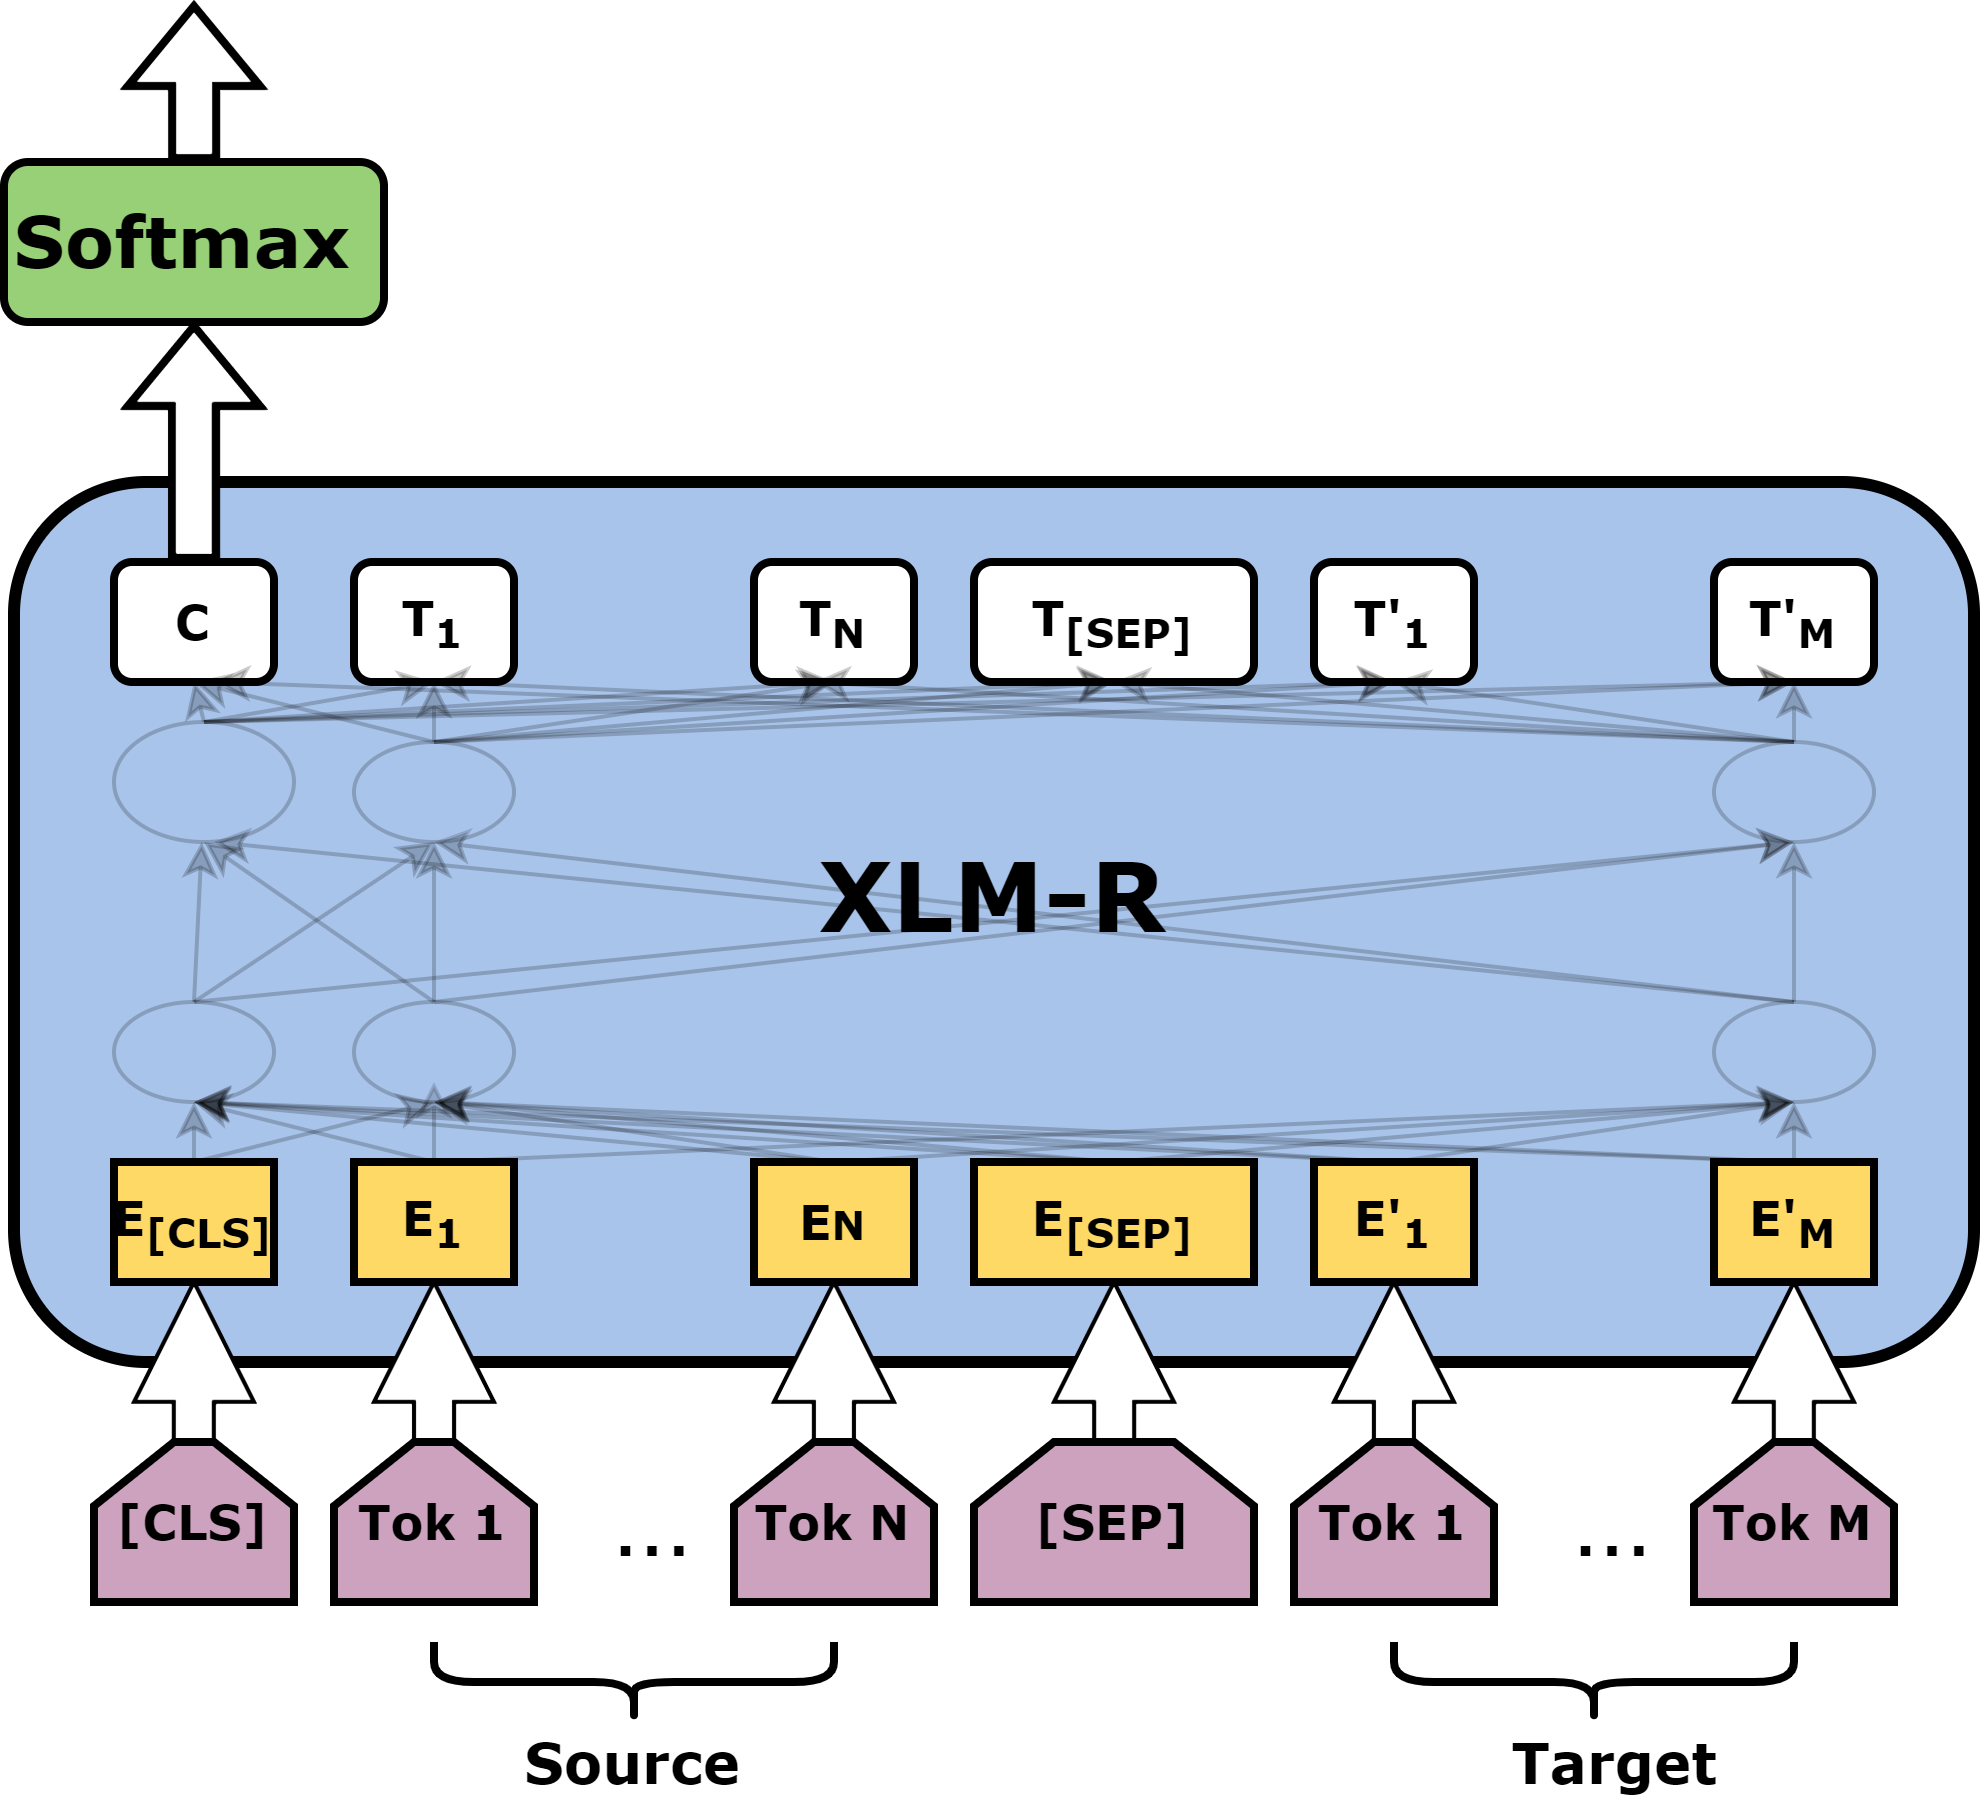
\includegraphics[width=8cm]{figures/translation_quality_estimation/transquest/TransQuest.png}
		\caption{\textit{MonoTransQuest} Architecture}
		\label{fig:monotransquest}
	\end{subfigure}
	\begin{subfigure}[b]{10cm}
		\centering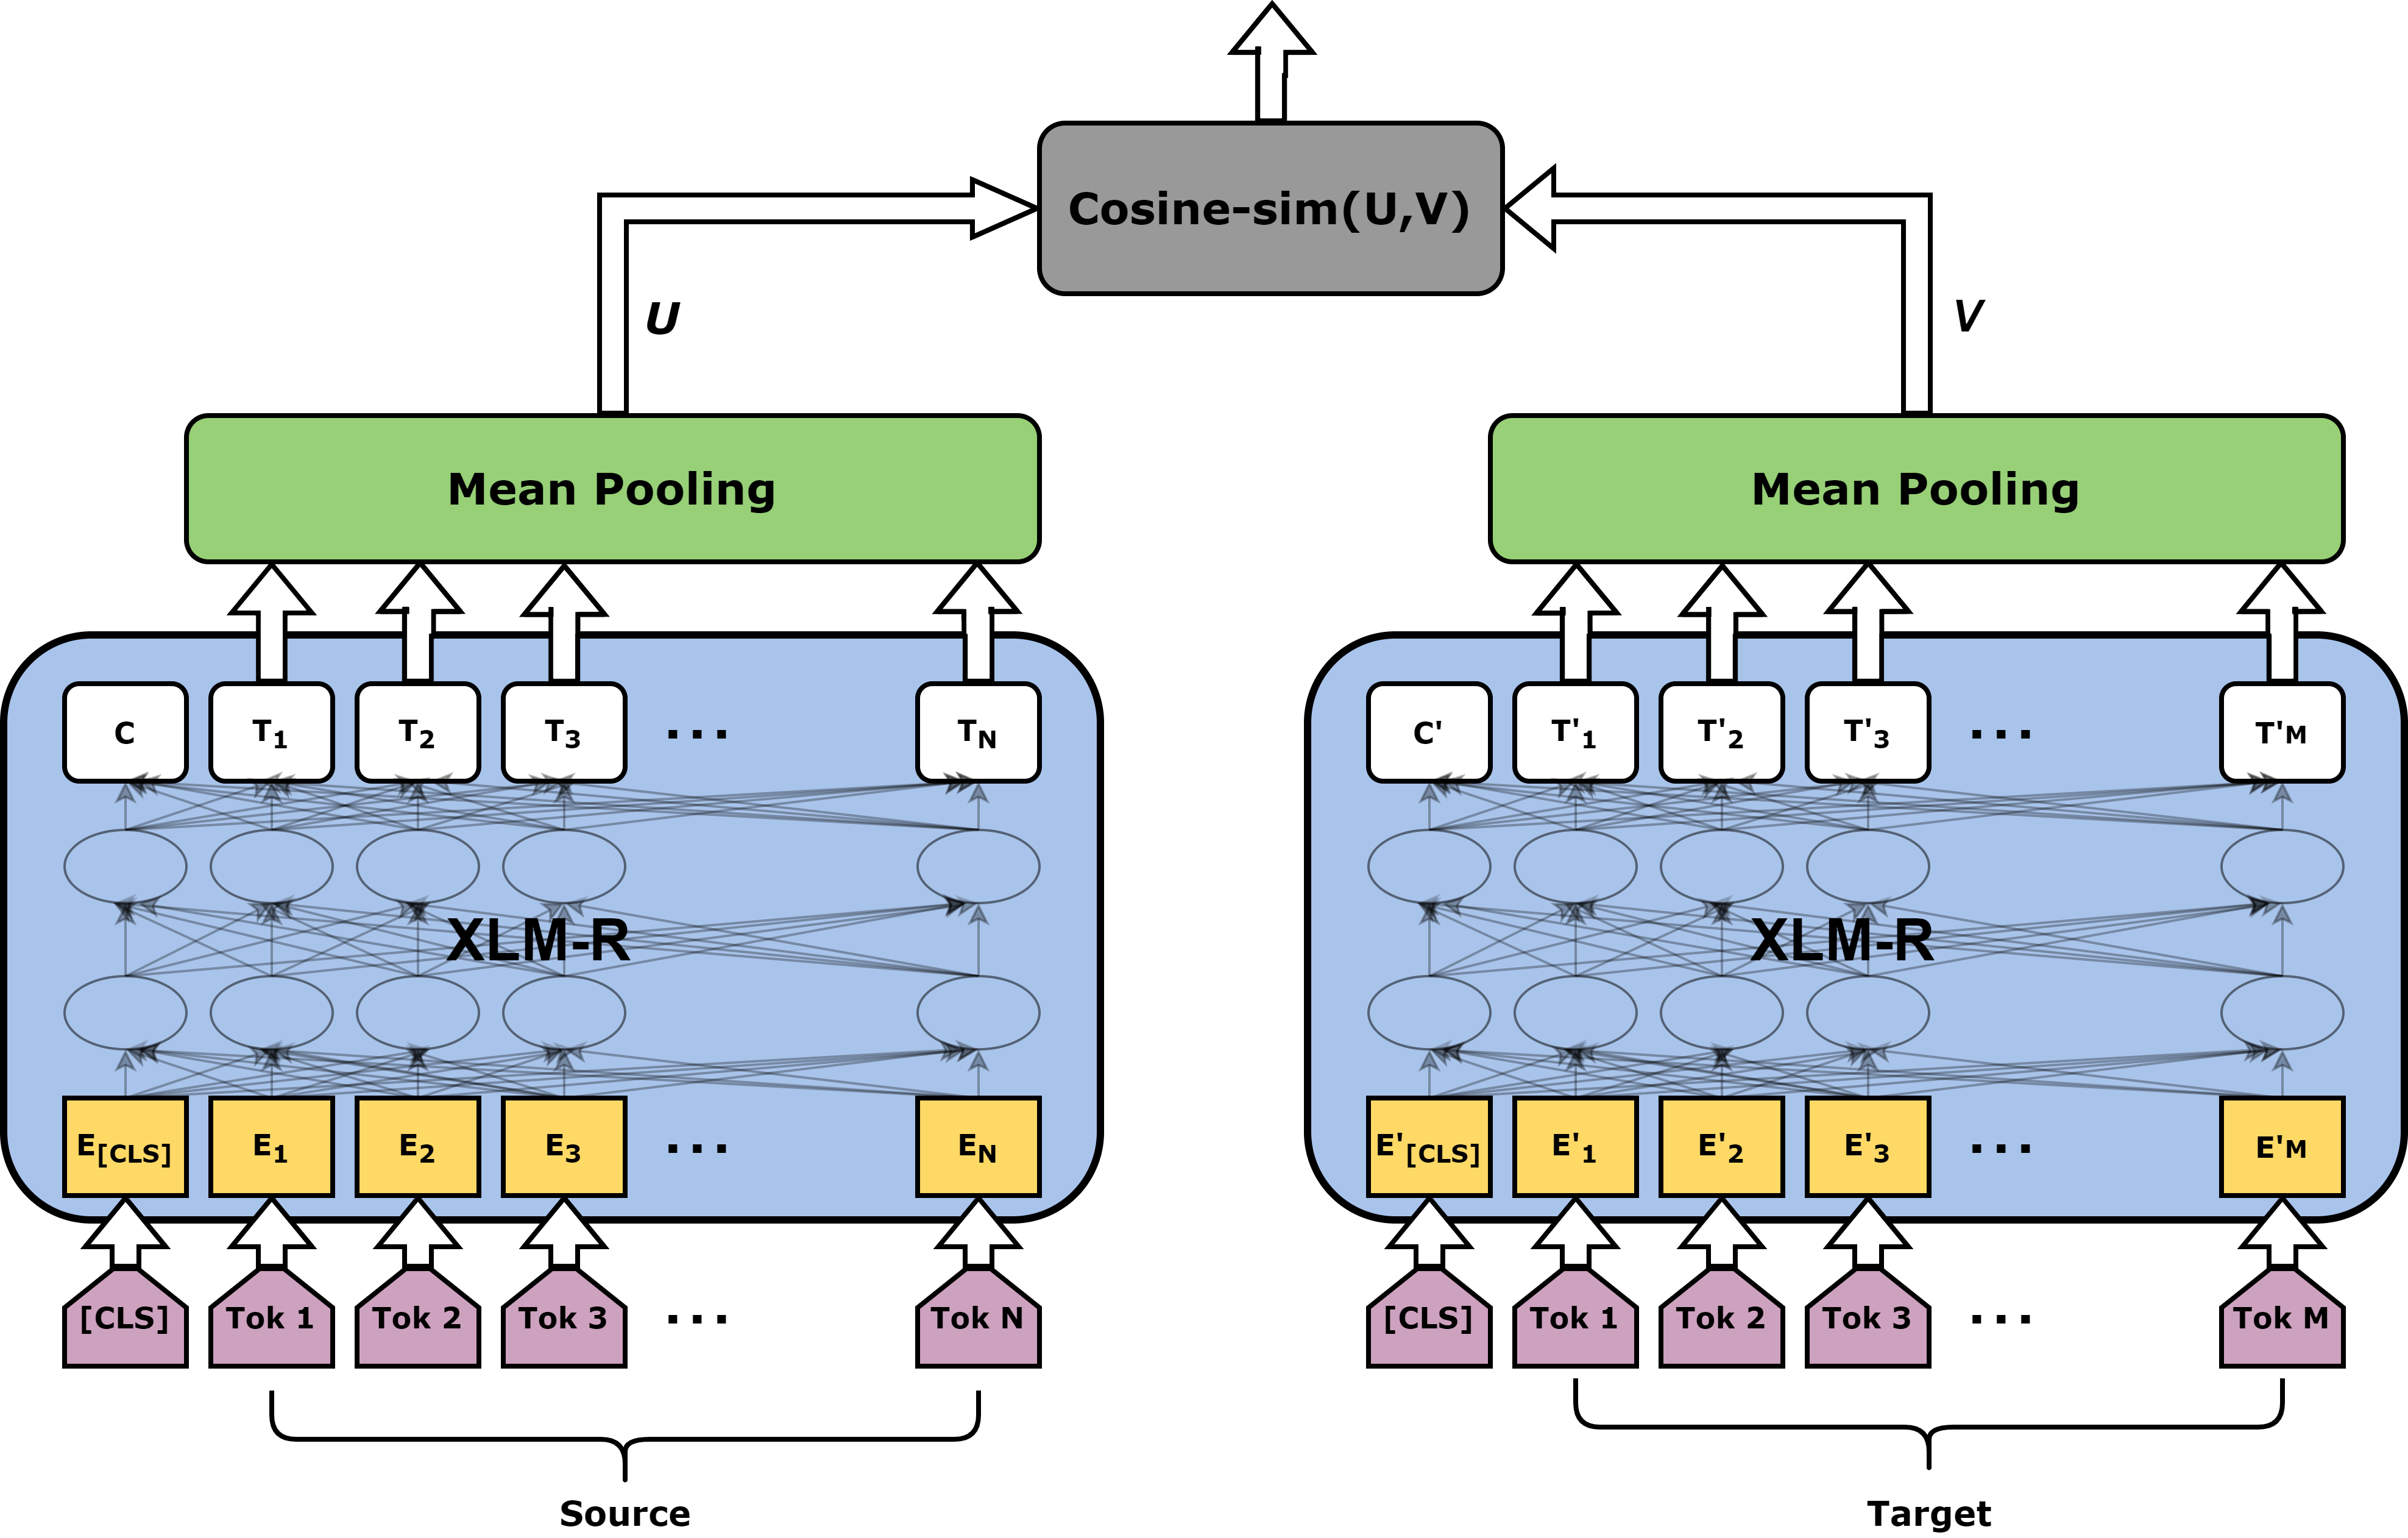
\includegraphics[width=12cm]{figures/translation_quality_estimation/transquest/SiameseTransQuest.png}
		\caption{\textit{SiameseTransQuest} Architecture}
		\label{fig:siamesetransquest}
	\end{subfigure}
	
	\caption[Architectures in TransQuest]{Two architectures employed in TransQuest.}
	\label{fig:transquest_architecture}
\end{figure}

\subsection{Experimental Setup}
\label{sec:transquest_experiment}
We evaluated these two architectures in both aspects of sentence-level quality estimation using the data introduced in Chapter \ref{cha:qe_introduction}. We applied the same set of configurations for all the language pairs in order to ensure consistency between all the experiments. This also provides a good starting configuration for researchers who intend to use TransQuest on a new language pair. In both architectures we used a batch-size of eight, Adam optimiser with learning rate $2\mathrm{e}{-5}$, and a linear learning rate warm-up over 10\% of the training data. During the training process, the parameters of XLM-R model, as well as the parameters of the subsequent layers, were updated. The models were trained using only training data. Furthermore, they were evaluated while training once in every 300 training steps using an evaluation set that had one fifth of the rows in training data. We performed early stopping if the evaluation loss did not improve over ten evaluation steps. All the models were trained for three epochs.

\section{Results and Discussion}
\label{sec:transquest_results}
The results for HTER and DA aspects are shown in Tables \ref{tab:hter_prediction} and \ref{tab:da_prediction}. We report the Pearson correlation ($\bm{\rho}$) between the predictions and the gold labels from the test set, which is the most commonly used evaluation metric in recent WMT quality estimation shared tasks \autocite{specia-etal-2018-findings,fonseca-etal-2019-findings,specia-etal-2020-findings-wmt} as mentioned in Chapter \ref{cha:qe_introduction}. Since we use the same evaluation process, we could compare our results with the baselines and best systems of the respective shared task. Raw I in Tables \ref{tab:hter_prediction} and \ref{tab:da_prediction} shows the results for MonTransQuest and SiameseTransQuest with XLM-R-large and Raw II in Tables \ref{tab:hter_prediction} and \ref{tab:da_prediction} shows the results for MonTransQuest and SiameseTransQuest with XLM-R-base. As can be seen in results XLM-R-large always outperformed XLM-R-base in both architectures. Therefore, we use the results we got from XLM-R-large for the following analysis.

\renewcommand{\arraystretch}{1.2}
\begin{table}[t]
	\begin{center}
		\small
		% \footnotesize
		\scalebox{0.8}{
		\begin{tabular}{l l  c c c c c c c c} 
			%\hline
			\toprule
			& & \multicolumn{4}{c}{\bf Mid-resource} & \multicolumn{4}{c}{\bf High-resource}\\\cmidrule(r){3-6}\cmidrule(r){7-10}
			&{\bf Method} & \makecell{En-Cs \\ SMT} & \makecell{ En-Ru \\ NMT} & \makecell{En-Lv \\ SMT} & \makecell{En-Lv \\ NMT} & \makecell{De-En \\ SMT} & \makecell{En-Zh \\ NMT} & \makecell{En-De \\ SMT } & \makecell{En-De \\ NMT} \\
			\midrule
			\multirow{2}{*}{\bf I} & MTransQuest & 0.7207 & 0.7126 & 0.6592 & 0.7394 & 0.7939 & 0.6119 & 0.7137 & 0.5994\\
			& STransQuest & 0.6853 & 0.6723 & 0.6320 & 0.7183 & 0.7524 & 0.5821& 0.6992 & 0.5875 \\
			\midrule
			\multirow{2}{*}{\bf II} & MTransQuest-base & 0.7012 & 0.6982 & 0.6254 & 0.7110 & 0.7653 & 0.5873 & 0.6872 & 0.5762 \\
			& STransQuest-base & 0.6678 & 0.6542 & 0.6132 & 0.6892 & 0.7251 & 0.5551 & 0.6672 & 0.5532 \\
			\midrule
			\multirow{2}{*}{\bf III} & MTransQuest $\otimes$ & 0.7300 & 0.7226 & 0.6601 & 0.7402 & 0.8021 & 0.6289 & 0.7289 & 0.6091 \\
			& STransQuest $\otimes$ & 0.6901 & 0.6892 & 0.6451 & 0.7251 & 0.7649 & 0.5967& 0.7041 & 0.5991 \\
			\midrule
			\multirow{2}{*}{\bf IV} & MTransQuest $\otimes$ - Aug & \textbf{0.7399} & \textbf{0.7307} & \textbf{0.6792} & \textbf{0.7492} & \textbf{0.8109} & 0.6367 & \textbf{0.7398} & 0.6156\\
			& STransQuest $\otimes$ - Aug & 0.7002 & 0.6901 & 0.6498 & 0.7301 & 0.7667 & 0.5991& 0.7134 & 0.6098 \\
			\midrule
			\multirow{3}{*}{\bf V} & Quest ++ & 0.3943 & 0.2601 & 0.3528 & 0.4435 & 0.3323 & NR & 0.3653 & NR \\
			& OpenKiwi & NR & 0.5923 & NR & NR & NR & 0.5058 & 0.7108 & 0.3923 \\
			& Best system & 0.6918 & 0.5923 & 0.6188 & 0.6819 & 0.7888 & \textbf{0.6641} & 0.7397 &  \textbf{0.7582} \\
			\midrule
			\multirow{2}{*}{\bf VI} & MTransQuest-B & 0.6423 & 0.6354 & 0.5772 & 0.6531 & 0.7005 & 0.5483 & 0.6239 & 0.5002 \\
			& STransQuest-B & 0.5987 & 0.5872 & 0.5012 & 0.5901 & 0.6572 & 0.5098& 0.5762 & 0.4551 \\
			\bottomrule
			%\bottomrule
		\end{tabular}
	}
	\end{center}
	\caption[Pearson correlation between TransQuest algorithm predictions and human post-editing effort]{Pearson correlation ($\bm{\rho}$) between \textit{TransQuest} algorithm predictions and human post-editing effort. Best results for each language by any method are marked in bold. Row I shows the results for XLM-R-large model and Row II shows the results for XLM-R-base. Row III and Row IV present the results for further fine-tuning strategies explained in Section \ref{sec:transquest_finetune}. Row V shows the results of the baseline methods and the best system submitted for the language pair in that competition. \textbf{NR} implies that a particular result was \textit{not reported} by the organisers. Row VI presents the results of the multilingual BERT (mBERT) model in TransQuest Architectures.} 
	\label{tab:hter_prediction}
\end{table}



\renewcommand{\arraystretch}{1.2}
\begin{table*}[t]
	\begin{center}
		\small
		\scalebox{0.85}{
		\begin{tabular}{l l  c c c c c c c} 
			%\hline
			\toprule
			& & \multicolumn{2}{c}{\bf Low-resource} & \multicolumn{3}{c}{\bf Mid-resource} & \multicolumn{2}{c}{\bf High-resource}\\\cmidrule(r){3-4}\cmidrule(lr){5-7}\cmidrule(l){8-9}
			&{\bf Method} & Si-En & Ne-En & Et-En & Ro-En & Ru-En & En-De & En-Zh\\
			\midrule
			\multirow{2}{*}{\bf I} & MTransQuest & 0.6525 & 0.7914 & 0.7748 & 0.8982 & 0.7734 & 0.4669 & 0.4779 \\
			& STransQuest & 0.5957 & 0.7081 & 0.6804 & 0.8501 & 0.7126 & 0.3992 & 0.4067 \\
			\midrule
			\multirow{2}{*}{\bf II} & MTransQuest-base & 0.6412 & 0.7823 & 0.7651 & 0.8715 & 0.7593 & 0.4421 & 0.4593 \\
			& STransQuest-base & 0.5773 & 0.6853 & 0.6692 & 0.8321 & 0.6962 & 0.3832 & 0.3975 \\
			\midrule
			\multirow{2}{*}{\bf III} & MTransQuest $\otimes$ & 0.6661 & 0.8023 & 0.7876 & 0.8988 & 0.7854 & 0.4862 & 0.4853 \\
			& STransQuest $\otimes$ & 0.6001 & 0.7132 & 0.6901 & 0.8629 & 0.7248 & 0.4096 & 0.4159 \\
			\midrule
			\multirow{2}{*}{\bf IV} & MTransQuest $\otimes$ - Aug & \textbf{0.6849} & \textbf{0.8222} & \textbf{0.8240} & \textbf{0.9082} & \textbf{0.8082} & \textbf{0.5539} & \textbf{0.5373} \\
			& STransQuest $\otimes$ - Aug & 0.6241 & 0.7354 & 0.7239 & 0.8621 & 0.7458 & 0.4457 & 0.4658 \\
			\midrule
			\multirow{1}{*}{\bf V} & OpenKiwi & 0.3737 & 0.3860 & 0.4770 & 0.6845 & 0.5479 & 0.1455 & 0.1902 \\
			\midrule
			\multirow{2}{*}{\bf VI} & MTransQuest-B & NS & 0.6452 & 0.6231 & 0.8351 & 0.6661 & 0.3765 & 0.3982  \\
			& STransQuest-B & NS & 0.5368 & 0.5431 & 0.7652& 0.5541 & 0.3356 & 0.3462 \\
			\bottomrule
		\end{tabular}
	}
	\end{center}
	\caption[Pearson correlation ($\bm{\rho}$) between \textit{TransQuest} algorithm predictions and human DA judgments]{Pearson correlation ($\bm{\rho}$) between \textit{TransQuest} algorithm predictions and human DA judgments. Best results for each language (any method) are marked in bold. Row I shows the results for XLM-R-large model and Row II shows the results for XLM-R-base. Row III and Row IV present the results for further fine-tuning strategies explained in Section \ref{sec:transquest_finetune}. Row V shows the results of the baseline method; OpenKiwi. Row VI presents the results of the multilingual BERT (mBERT) model in TransQuest Architectures.} 
	\label{tab:da_prediction}
\end{table*}

In the HTER aspect of sentence-level quality estimation, as shown in Table \ref{tab:hter_prediction}, \textit{MonoTransQuest} gains $\approx$ 0.1-0.2 Pearson correlation boost over OpenKiwi in most language pairs. In the language pairs where OpenKiwi results are not available \textit{MonoTransQuest} gains $\approx$ 0.3-0.4 Pearson correlation boost over QuEst++ in all language pairs for both NMT and SMT. Table \ref{tab:hter_prediction}  also gives the results of the best system submitted for a particular language pair. It is worth noting that the \textit{MonoTransQuest} results surpass the best system in all the language pairs with the exception of the En-De SMT, En-De NMT and En-Zh NMT datasets. \textit{SiameseTransQuest} fall behind \textit{MonoTransQuest} architecture, however still it outperforms OpenKiwi and Quest++ in all the language pairs except En-De SMT. This shows that simple STS models with crosslingual embeddings outperforms the complex state-of-the-art QE models in predicting HTER. 


As shown in Table \ref{tab:da_prediction}, in the DA aspect of quality estimation, \textit{MonoTransQuest}  gained $\approx$ 0.2-0.3 Pearson correlation boost over OpenKiwi in all the language pairs. Additionally, \textit{MonoTransQuest} achieves $\approx$ 0.4 Pearson correlation boost over OpenKiwi in the low-resource language pair Ne-En. Similar to HTER, in DA too \textit{SiameseTransQuest} fall behind \textit{MonoTransQuest} architecture, however still \textit{SiameseTransQuest} 
gained $\approx$ 0.2-0.3 Pearson correlation boost over OpenKiwi in all the language pairs. This shows that simple STS models with crosslingual embeddings outperforms the complex state-of-the-art QE models in predicting DA too.


If you consider the two architectures; \textit{MonoTransQuest} and \textit{SiameseTransQuest}, \textit{MonoTransQuest} outperformed the \textit{SiameseArchitecture} in all the language pairs in both aspects of sentence-level quality estimation. This is inline with the experiments we discussed for monolingual STS in Part I of the thesis. The two architectures have a trade-off between accuracy and efficiency. On an Nvidia Tesla K80 GPU, \textit{MonoTransQuest} takes 4,480s on average to train on 7,000 instances, while \textit{SiameseTransQuest} takes only 3,900s on average for the same experiment. On the same GPU, \textit{MonoTransQuest} takes 35s on average to perform inference on 1,000 instances which takes \textit{SiameseTransQuest} only 16s to do so. Therefore we recommend using \textit{MonoTransQuest} where accuracy is valued over efficiency, and \textit{SiameseTransQuest} where efficiency is prioritised above accuracy. Furthermore, as we discussed in Part I of the thesis, Siamese architecture outputs sentence vectors. Therefore finding the best quality translation in a collection of translations would take a less time with the Siamese architecture. Since there is a growing interest\footnote{Several workshops like $EMC^2$ (Workshop on Energy Efficient Machine Learning and Cognitive Computing), SustaiNLP 2020 (Workshop on Simple and Efficient Natural Language Processing) has been organised on this aspect.} in the NLP community for energy efficient machine learning models, we decided to support both architectures in the TransQuest Framework. 

With these results we can answer our \textbf{RQ1:} Can the state-of-the-art STS models applied in sentence-level QE task by changing the embeddings? We show that state-of-the-art STS methods based on crosslingual transformer models outperform current state-of-the-art QE algorithms based on complex architectures like predictor-estimator in both aspects of sentence-level QE. We support this with the results for more than 15 language pairs with a wide variety from different domains and different MT types.


Additionally, Row VI in both Tables \ref{tab:hter_prediction} and \ref{tab:da_prediction} shows the results of multilingual BERT (mBERT) in MonoTransQuest and SiameseTransQuest architecture. We used the same settings similar to XLM-R. The results show that XLM-R model outperforms the mBERT model in all the language pairs of both aspects in quality estimation. As shown in row II in both Tables \ref{tab:hter_prediction} and \ref{tab:da_prediction} even XLM-R-base model outperform mBERT model in all the languages pairs with both architectures. Therefore, we can safely assume that the cross lingual nature of the XLM-R transformers had a clear impact to the results.

With this we can answer our \textbf{RQ2:} Using crosslingual embeddings with STS architecture proved advantageous rather than using just multilingual embeddings. Therefore, state-of-the-art crosslingual transformer models like XLM-R should be utilised in QE tasks more. 


\section{Further Fine-tuning}
\label{sec:transquest_finetune}
In this section. we try improve the results of TransQuest through two fine-tuning strategies; ensemble learning and data augmentation. 

\paragraph{Ensemble Learning} uses multiple learning algorithms to obtain better predictive performance than could be obtained from any of the constituent learning algorithms alone. We perform a weighted average ensemble for the output of the XLM-R-large and the output of the XLM-R-base for both architectures in TransQuest. We experimented on weights 0.8:0.2, 0.6:0.4, 0.5:0.5 on the output of XLM-R-large and output from XLM-R-base respectively. Since the results we got from XLM-R-base transformer model are slightly worse than the results we got from XLM-R-large we did not consider the weight combinations that gives higher weight to XLM-R-base transformer model results. We obtained best results when we used the weights 0.8:0.2. We report the results from the two architectures from this step in row III of Tables \ref{tab:hter_prediction} and \ref{tab:da_prediction} as MTransQuest $\otimes$ and STransQuest $\otimes$.

As shown in Tables \ref{tab:hter_prediction} and \ref{tab:da_prediction} both architectures in TransQuest with ensemble learning gained $\approx$ 0.01-0.02 Pearson correlation boost over the default settings for all the language pairs in both aspects of sentence-level QE.  

\paragraph{Data Augmentation} adds additional training instances for the training process. As we already experienced with STS experiments in Part I of the thesis, this often leads to better performance of the machine learning algorithms. Therefore, to experiment how TransQuest performs with more data, we trained TransQuest on a data augmented setting. Alongside the training, development and testing datasets, the shared task organisers also provided the parallel sentences which were used to train the neural machine translation system in each language. In the data augmentation setting, we added the sentence pairs from that neural machine translation system training file to training dataset we used to train TransQuest. In order to find the best setting for the data augmentation we experimented with adding 1000, 2000, 3000, up to 5000 sentence pairs randomly. Since the ensemble learning performed better than XLM-R large results of TransQuest, we conducted this data augmentation experiment on the ensemble learning setting. We assumed that the sentence pairs added from the neural machine translation system training file have maximum translation quality. 

Up to 2000 sentence pairs the results continued to get better. However, adding more than 2000 sentence pairs did not improve the results. We did not experiment with adding any further than 5000 sentence pairs to the training set since we were aware that adding more sentence pairs with the maximum translation quality to the training file will make it imbalance and affect the performance of the machine learning models negatively. We report the results from the two architectures from this step in row IV of Tables \ref{tab:hter_prediction} and \ref{tab:da_prediction} as MTransQuest $\otimes$-Aug and STransQuest $\otimes$-Aug. 

Data augmentation provided the best results for all of the language pairs in both aspects of sentence-level QE. As shown in Tables \ref{tab:hter_prediction} and \ref{tab:da_prediction} both architectures in TransQuest with the data augmentation setting gained $\approx$ 0.01-0.09 Pearson correlation boost over the XLM-R-large all the language pairs. Additionally for DA, \textit{MTransQuest $\otimes$-Aug} achieves $\approx$ 0.09 Pearson correlation boost over TransQuest with XLM-R large in the high-resource language pair En-De which is the biggest boost got for any language pair. 

This answers our \textbf{RQ3:} Can further fine-tuning strategies used to improve the results? We show that ensemble learning and 
data augmentation can be used improve the results. In fact, data augmentation combined with ensemble learning provided best results for all the language pairs in both aspects of the sentence-level QE. 

Finally, we submitted the best result we had with TransQuest (MonoTransQuest with ensemble learning and data augmentation) to WMT 2020 QE shared task 1 \autocite{specia-etal-2020-findings-wmt}. The official results of the competition show that \textit{TransQuest} won the first place in all the language pairs in Sentence-Level Direct Assessment task. \textit{TransQuest} is the sole winner in En-Zh, Ne-En and Ru-En language pairs and the multilingual track. For the other language pairs (En-De, Ro-En, Et-En and Si-En) it shares the first place with \autocite{fomicheva-etal-2020-bergamot}, whose results are not statistically different from ours. Therefore, TransQuest is the new state-of-the-art in sentence-level QE.

\section{Error analysis}
\label{sec:transquest_error}

In an attempt to better understand the performance and limitations of \textit{TransQuest} we carried out an error analysis on the results obtained on Romanian - English and Sinhala - English. The choice of language pairs we analysed was determined by the availability of native speakers to perform this analysis. We focused on the cases where the difference between the predicted score and expected score was the greatest. This included both cases where the predicted score was underestimated and overestimated. 

Analysis of the results does not reveal very clear patterns. The largest number of errors seem to be caused by the presence of named entities in the source sentences. In some cases these entities are mishandled during the translation. The resulting sentences are usually syntactically correct, but semantically odd. Typical examples are \emph{RO: În urmă explorărilor Căpitanului James Cook, Australia și Noua Zeelandă au devenit ținte ale colonialismului britanic. (As a result of Captain James Cook's explorations, Australia and New Zealand have  become the targets of British colonialism.)} - \emph{EN: Captain James Cook, Australia and New Zealand have finally become the targets of British colonialism.} (expected: -1.2360, predicted: 0.2560) and \emph{RO: O altă problemă importantă cu care trupele Antantei au fost obligate să se confrunte a fost malaria. (Another important problem that the Triple Entente troops had to face was malaria.)} - EN: \emph{Another important problem that Antarctic troops had to face was malaria.} (expected: 0.2813, predicted: -0.9050). 
In the opinion of the authors of this paper, it is debatable whether the expected scores for these two pairs should be so different. Both of them have obvious problems and cannot be clearly understood without reading the source. For this reason, we would expect that both of them have low scores. Instances like this also occur in the training data. As a result of this, it may be that \textit{TransQuest} learns contradictory information, which in turn leads to errors at the testing stage.

A large number of problems are caused by incomplete source sentences or input sentences with noise. For example the pair \emph{RO: thumbright250pxDrapelul cu fâșiile în poziție verticală (The flag with strips in upright position)} -  \emph{EN: ghtghtness 250pxDrapel with strips in upright position} has an expected score of 0.0595, but our method predicts -0.9786. Given that only \emph{ghtghtness 250pxDrapel} is wrong in the translation, the predicted score is far too low. In an attempt to see how much this noise influences the result, we run the system with the pair \emph{RO: Drapelul cu fâșiile în poziție verticală} -  \emph{EN: Drapel with strips in upright position}. The prediction is 0.42132, which is more in line with our expectations given that one of the words is not translated. 

Similar to Ro-En, in Si-En the majority of problems seem to be caused by the presence of named entities in the source sentences. For an example in the English translation: \emph{But the disguised Shiv will help them securely establish the statue.
} (expected: 1.3618, predicted: -0.008), the correct English translation would be \emph{But the disguised Shividru will help them securely establish the statue.}. Only the named entity \emph{Shividru} is translated incorrectly, therefore the annotators have annotated the translation with a high quality. However TransQuest fails to identify that. Similar scenarios can be found in English translations \emph{Kamala Devi Chattopadhyay spoke at this meeting, Dr. Ann.} (expected:1.3177, predicted:-0.2999) and \emph{The Warrior Falls are stone's, halting, heraldry and stonework rather than cottages. The cathedral manor is navigable places} (expected:0.1677, predicted:-0.7587). It is clear that the presence of the named entities seem to confuse the algorithm we used, hence it needs to handle named entities in a proper way.


\section{Conclusion}
\label{sec:transquest_conclusion}
In this paper we introduced \textit{TransQuest}, a new open source framework for quality estimation based on cross-lingual transformers. \textit{TransQuest} is implemented using PyTorch \autocite{NEURIPS2019_9015} and HuggingFace \autocite{wolf-etal-2020-transformers} and supports training of sentence-level quality estimation systems on new data. It outperforms other open-source tools on both aspects of sentence-level quality estimation and yields new state-of-the-art quality estimation results. 


We propose two architectures: \textit{MonoTransQuest} and \textit{SiameseTransQuest}. As we showed in Part I of the thesis, they provide state-of-the-art results for STS. However, neither of them have been previously explored in QE tasks. As far as we know, it is the first time that STS architectures have been proposed to the QE task. We further improve the results with data augmentation and ensemble learning. The best results we achieved in this chapter were submitted to WMT 2020 QE task 1 and it won the first place in all the language pairs. We can conclude that TransQuest is the state-of-the-art in QE now.

We have open-sourced the framework and the pre-trained sentence-level QE models for 15 language pairs are freely available to the community in HuggingFace model hub. Upon releasing TransQuest has caught a wide attention from the community resulting in more than 9,000 downloads within the first year. Furthermore, TransQuest has been used as the baselines for many shared tasks including the most recent edition of WMT QE shared task\footnote{WMT 2021 QE shared task is available on \url{http://statmt.org/wmt21/quality-estimation-task.html}} and Explainable Quality Estimation shared task on the second workshop on Evaluation \& Comparison of NLP Systems\footnote{Explainable Quality Estimation shared task is available on \url{https://eval4nlp.github.io/sharedtask.html}}. Not only among researches, TransQuest is popular among the industry too. ModelFront, which is a leading company in translation risk prediction lists TransQuest as an option in their website\footnote{ModelFront options are available on \url{https://modelfront.com/options}}. We believe that the simplicity of the architectures in TransQuest is the reason for this popularity. 

Sentence-level QE models are difficult to interpret as they only provide a score for the whole translation without indicating where the errors are. To overcome this with TransQuest, we introduce minor changes to the sentence-level architecture to support word-level quality estimation in Chapter \ref{cha:qe_word}. One limitation with TransQuest is that the pre-trained QE models are big in size as they depend on transformer models. Therefore, managing a several of them for each language pair would be chaotic in a real-world application. We seek solutions for that with multilingual QE models in Chapter \ref{cha:qe_multilingual}. 

As future work, we hope to explore crosslingual embeddings more with TransQuest for the sentence-level QE task. For an example XeroAlign \autocite{gritta-iacobacci-2021-xeroalign} provides a simple method for task-specific alignment of crosslingual pre-trained transformers which would be interesting to apply in QE task too. Furthermore, Facebook has introduced large crosslingual models recently; XLM-R XL and XLM-R XXL which have improved results for many crosslingual NLP tasks \autocite{goyal2021}. These models have obvious disadvantage of being big in size; yet would be interesting to apply in QE. 









